\section{Data sources}\label{sec:sources}

Report cards are typically compiled and communicated annually.  However, the time window that
constitutes a year differs from report card to report card.  Many environmental report cards
communicate on data collected within a financial year.  This schedule provides a reporting window
that is consistent with other management and governmental considerations.  Others use a time window
that naturally aligns with the cycle of some major underlying environmental gradient - such as
wet/dry season. For this project, we are adopting using the same water year (1st Oct -- 30 Sept)
definition as the AIMS inshore Water Quality Marine Monitoring Program \citep{Lonborg-MMP-2015}.

The Great Barrier Reef Marine Park (GBR), spans nearly 14$^\circ$ of latitude, covers approximately
344,400km$^2$ and in so doing spans multiple jurisdictions with differing pressures and management strategies.
Furthermore, the GBR also spans a substantial longitudinal range being bounded by the Queesland coastline in the west and the outer reef in the east.
Hence, it is useful to partition
the GBR into smaller more homogeneous zones representing combinations of region and water body.
For this project, we will adopt
six regions (Cape York, Wet Tropics, Dry Tropics, Mackay Whitsunday, Fitzroy and Burnett Mary) and
four water bodies (Enclosed Coastal, Open Coastal, Midshelf and Offshore), see Figure \ref{fig:Map_region_waterbody}.
Following the recomendations of the Idependent Science Panel (ISP), the Enclosed Coastal zone will be
excluded from the majority of high level summary products.  Nevertheless, it will be present in exploratory
data analysis products for the sake of transparency as well as to provide some form of validation and
justification for ISP's recommendations.
 
  \arrayrulecolor[rgb]{0.06,0.25,0.49}
 \LTcapwidth=\linewidth
 \setlength\aboverulesep{0pt}\setlength\belowrulesep{0pt}
 \setlength\cmidrulekern{1pt}\setlength\cmidrulewidth{1pt}
 \renewcommand\arraystretch{1.2}\setlength\tabcolsep{5pt}
 %\begin{landscape}
 \begin{table}[h]\caption{Great Barrier Reef spatial Zones and associated Regions and Water bodies.}\label{tab:spatial}
 %\begin{center}
 \scriptsize
 \begin{tabular}{
 !{\color[rgb]{0.06,0.25,0.49}\VRule[1pt]} p{25em}
 !{\color[rgb]{0.06,0.25,0.49}\vline} l
 !{\color[rgb]{0.06,0.25,0.49}\vline} l
 !{\color[rgb]{0.06,0.25,0.49}\vline} l
 !{\color[rgb]{0.06,0.25,0.49}\VRule[1pt]}
 }
 \arrayrulecolor[rgb]{0.06,0.25,0.49}\specialrule{1pt}{0pt}{0pt} %top border
 \rowcolor[rgb]{0.53,0.62,0.74} 
 %\multicolumn{1}{!{\color[rgb]{0.06,0.25,0.49}\VRule[1pt]}l}}{\whiteHeader{{GBRMPA Zone}}} & 
 \multicolumn{1}{l}{\whiteHeader{{GBRMPA Zone}}} & 
 \multicolumn{1}{l}{\whiteHeader{{Zone}}} & 
 \multicolumn{1}{l}{\whiteHeader{{Region}}} & 
 \whiteHeader{{Water body}}\\ 
 \cmidrule{1-4} 
Enclosed\_Coastal\_Cape\_York & Enclosed\_Coastal\_Cape York & Cape York & Enclosed Coastal \\ 
  Enclosed\_Coastal\_Terrain\_NRM & Enclosed\_Coastal\_Wet Tropics & Wet Tropics & Enclosed Coastal \\ 
  Enclosed\_Coastal\_Burdekin\_Dry\_Tropics\_NRM & Enclosed\_Coastal\_Dry Tropics & Dry Tropics & Enclosed Coastal \\ 
  Enclosed\_Coastal\_Mackay\_Whitsunday\_NRM\_Group & Enclosed\_Coastal\_Mackay Whitsunday & Mackay Whitsunday & Enclosed Coastal \\ 
  Enclosed\_Coastal\_Fitzroy\_Basin\_Association & Enclosed\_Coastal\_Fitzroy & Fitzroy & Enclosed Coastal \\ 
  Enclosed\_Coastal\_Burnett\_Mary\_Regional\_Group\_for\_NRM & Enclosed\_Coastal\_Burnett Mary & Burnett Mary & Enclosed Coastal \\ 
   \cline{1-4}Open\_Coastal\_Cape\_York & Open\_Coastal\_Cape York & Cape York & Open Coastal \\ 
  Open\_Coastal\_Terrain\_NRM & Open\_Coastal\_Wet Tropics & Wet Tropics & Open Coastal \\ 
  Open\_Coastal\_Burdekin\_Dry\_Tropics\_NRM & Open\_Coastal\_Dry Tropics & Dry Tropics & Open Coastal \\ 
  Open\_Coastal\_Mackay\_Whitsunday\_NRM\_Group & Open\_Coastal\_Mackay Whitsunday & Mackay Whitsunday & Open Coastal \\ 
  Open\_Coastal\_Fitzroy\_Basin\_Association & Open\_Coastal\_Fitzroy & Fitzroy & Open Coastal \\ 
  Open\_Coastal\_Burnett\_Mary\_Regional\_Group\_for\_NRM & Open\_Coastal\_Burnett Mary & Burnett Mary & Open Coastal \\ 
   \cline{1-4}Midshelf\_Cape\_York & Midshelf\_Cape York & Cape York & Midshelf \\ 
  Midshelf\_Terrain\_NRM & Midshelf\_Wet Tropics & Wet Tropics & Midshelf \\ 
  Midshelf\_Burdekin\_Dry\_Tropics\_NRM & Midshelf\_Dry Tropics & Dry Tropics & Midshelf \\ 
  Midshelf\_Mackay\_Whitsunday\_NRM\_Group & Midshelf\_Mackay Whitsunday & Mackay Whitsunday & Midshelf \\ 
  Midshelf\_Fitzroy\_Basin\_Association & Midshelf\_Fitzroy & Fitzroy & Midshelf \\ 
  Midshelf\_Burnett\_Mary\_Regional\_Group\_for\_NRM & Midshelf\_Burnett Mary & Burnett Mary & Midshelf \\ 
   \cline{1-4}Offshore\_Cape\_York & Offshore\_Cape York & Cape York & Offshore \\ 
  Offshore\_Terrain\_NRM & Offshore\_Wet Tropics & Wet Tropics & Offshore \\ 
  Offshore\_Burdekin\_Dry\_Tropics\_NRM & Offshore\_Dry Tropics & Dry Tropics & Offshore \\ 
  Offshore\_Mackay\_Whitsunday\_NRM\_Group & Offshore\_Mackay Whitsunday & Mackay Whitsunday & Offshore \\ 
  Offshore\_Fitzroy\_Basin\_Association & Offshore\_Fitzroy & Fitzroy & Offshore \\ 
  Offshore\_Burnett\_Mary\_Regional\_Group\_for\_NRM & Offshore\_Burnett Mary & Burnett Mary & Offshore \\ 
   \bottomrule
 \end{tabular}
 %\end{center}
 \end{table} %\end{landscape}


  
\begin{figure}[ptbh] \includegraphics[width=1\linewidth]{figures/Maps/Map_region_waterbody\res.pdf}
\caption{Great Barrier Reef Zones (Regions and Water Bodies).}\label{fig:Map_region_waterbody}
\end{figure}
   
  \arrayrulecolor[rgb]{0.06,0.25,0.49}
 \LTcapwidth=\linewidth
 \setlength\aboverulesep{0pt}\setlength\belowrulesep{0pt}
 \setlength\cmidrulekern{1pt}\setlength\cmidrulewidth{1pt}
 \renewcommand\arraystretch{1.2}\setlength\tabcolsep{5pt}
 \begin{table}[h]\caption{Summary of used data sources.}\label{tab:sources}
 %\begin{center}
 \scriptsize
 \begin{tabular}{
 !{\color[rgb]{0.06,0.25,0.49}\VRule[1pt]} p{6em}
 !{\color[rgb]{0.06,0.25,0.49}\vline} l
 !{\color[rgb]{0.06,0.25,0.49}\vline} l
 !{\color[rgb]{0.06,0.25,0.49}\VRule[1pt]}
 }
 \arrayrulecolor[rgb]{0.06,0.25,0.49}\specialrule{1pt}{0pt}{0pt} %top border
 \rowcolor[rgb]{0.53,0.62,0.74} 
 \multicolumn{1}{!{\color[rgb]{0.06,0.25,0.49}\VRule[1pt]}l}{\whiteHeader{{Source}}} & 
 \multicolumn{1}{l}{\whiteHeader{{Custodian}}} & 
 \whiteHeader{{Description}}\\ 
 \cmidrule{1-3} 
AIMS Insitu & AIMS & AIMS inshore monitoring program Niskin data \\ 
   \cline{1-3}AIMS FLNTU & AIMS & AIMS inshore monitoring program FLNTU logger data \\ 
   \cline{1-3}Satellite & BOM & BOM: Catalog http://ereeftds.bom.gov.au/ereefs/tds/catalog/ereef/mwq/P1D/2002/catalog.html \\ 
   \cline{1-3}eReefs & eReefs & \textcolor{red}{provide a description in ../parameters/sources.csv} \\ 
   \cline{1-3}eReefs926 & eReefs & eReefs: http://dapds00.nci.org.au/thredds/catalog/fx3/gbr4\_bgc\_926/catalog.html \\ 
   \bottomrule
 \end{tabular}
 %\end{center}
 \end{table}

 

\subsection{Indicators}

One of the biggest challenges of report card development is the selection of appropriate indicators
from amongst a potentially very large candidate pool.  Since the outcomes, conclusions and
implications are all dependent on the indicators selected, the selection process is one of the most
influential steps and has justifiably received a great deal of attention.

As part of their ecosystem report card framework, \citet{Harwell-1999} urged that the alignment of
scientific information with societal goals and objectives should be the guiding principle of
indicator selection.  In their framework, clearly articulated societal goals and objectives (a
combination of societal values and scientific knowledge, such as restored and sustainable wetland
system) are translated into Essential Ecosystem Characteristics (EECs) that represent a set of
generic attributes that further refine the broad goals (such as water quality, sediment quality,
habitat quality, ecological processes).  The EEC's are then further translated into a set of
scientific informed indicators that are measured or monitored to indicate the status of trends or
states associated with the EEC's.
  
There have since been numerous studies that have focused on providing more formal, objective
criterion for indicator selection \citep{Dauvin-2008, Emerson-2012, Flint-2012, James-2012}.  Whilst
the specifics vary, most can be broadly encapsulated by a \citet{Dauvin-2008}'s contextual
implementation of the \citet{Doran-1981}'s SMART (Simple, Measurable, Achievable, Realistic, and
Time limited) principle.  A 'good' indicator should be representative, easily interpreted, broadly
comparable, sensitive to change and have a reference or guideline value.  To be `useful', an
indicator must be approved by international consensus, be well grounded and documented, have a
reasonable cost/benefit ratio and have adequate historical and on-going spatial-temporal coverage.
\citet{Flint-2012} and \citet{James-2012} further developed numerical scoring systems to help
evaluate indicators objectively.  Nevertheless, \citep{Neary-2012} warned against the potential to
manipulate an index by saturating with inappropriate or biased indicators and whilst recommending
that an index comprise of at least seven indicators, they did advocate that the type of indicator is
more important than the number of indicators._

Since final outcomes are likely to be highly influenced by indicator choice, the robustness and
sensitivity of both indicators and final outcomes to changes in ecosystem health should be
understood if not formally investigated as part of the indicator selection process
\citep{Dobbie-2013}.  Sensitivity analyses can involve:

\begin{itemize}
\item simulating changes in the underlying data of different magnitudes and estimating the resulting
sensitivity (percentage or probability of change) expressed by the indicator
\item estimating the effect of past perturbations on the indicator hindcasted from on historical
data
\end{itemize}

As stressed above, indicators should align intimately with report card objectives.  Yet in the more
broad ecosystem report card frameworks, such indicators are often too general to be measurable.
Therefore, in such cases, the indicators are further sub-divided into progressively more specific
measures.  For example, an indicator of water quality might comprise sub-indicators of nutrients,
metals and physico-chemistry which in turn might be represented by more specific measures such as
total nitrogen, mercury, dissolved oxygen, pH etc.

The resulting design is a hierarchical structure in which sub-indicators (etc) are nested within
indicators and spatial scales are nested from entire regions, sub-regions or zones down to
individual sites or sampling units.  One of the strengths of such a hierarchical report card
framework is that the inherent inbuilt redundancy allows for the addition, deletion or exchange of
finer scale items (sites and actual measured variables) with minimum disruption to the actual report
indicators.  That is, the indicator is relatively robust to some degree of internal makeup.
Furthermore, by abstracting away the fine details of an indicator, similar indicators from different
report cards (each potentially comprising different sampling designs) are more directly comparable.
For example, in different report cards that include water quality, a water quality indicator of
'water clarity' might comprise different Measures (e.g. suspended solids, NTU, Secchi depth etc)
collected from different sources (e.g. satellite, in situ loggers or hand samples), yet provided
each of these water clarity indicators are well calibrated, it should be possible to compare state
and trend across the report cards.
  
  \arrayrulecolor[rgb]{0.06,0.25,0.49}
 \LTcapwidth=\linewidth
 \setlength\aboverulesep{0pt}\setlength\belowrulesep{0pt}
 \setlength\cmidrulekern{1pt}\setlength\cmidrulewidth{1pt}
 \renewcommand\arraystretch{1.2}\setlength\tabcolsep{5pt}
 \begin{table}[h]\caption{Water Quality Measure hierarchy specifying which Measures contribute to which Subindicators and which Subindicators contribute to which Indicators.}\label{tab:measures}
 \begin{center}
 \scriptsize
 \begin{tabular}{
 !{\color[rgb]{0.06,0.25,0.49}\VRule[1pt]} p{6em}
 !{\color[rgb]{0.06,0.25,0.49}\vline} l
 !{\color[rgb]{0.06,0.25,0.49}\vline} l
 !{\color[rgb]{0.06,0.25,0.49}\vline} l
 !{\color[rgb]{0.06,0.25,0.49}\vline} l
 !{\color[rgb]{0.06,0.25,0.49}\VRule[1pt]}
 }
 \arrayrulecolor[rgb]{0.06,0.25,0.49}\specialrule{1pt}{0pt}{0pt} %top border
 \rowcolor[rgb]{0.53,0.62,0.74} 
 \multicolumn{1}{!{\color[rgb]{0.06,0.25,0.49}\VRule[1pt]} p{6em}}{\whiteHeader{{Indicator}}} & 
 \multicolumn{1}{l}{\whiteHeader{{Subindicator}}} & 
 \multicolumn{1}{l}{\whiteHeader{{Measure}}} & 
 \multicolumn{1}{l}{\whiteHeader{{Label}}} & 
 \whiteHeader{{Units}}\\ 
 \cmidrule{1-5} 
 \cline{1-5}Water Quality & Productivity & chl & Chlorophyll & µgL^{-1} \\ 
   \cline{3-5} \cline{2-5}Water Quality & Water Clarity & nap & TSS & mgL^{-1} \\ 
   \cline{3-5}Water Quality & Water Clarity & ntu & NTU & NTU \\ 
   \cline{3-5}Water Quality & Water Clarity & sd & Secchi & m \\ 
   \cline{3-5} \cline{2-5}Water Quality & Nutrients & NOx & NOx & µgL^{-1} \\ 
   \bottomrule
 \end{tabular}
 \end{center}
 \end{table}
   
   
  
\subsection{AIMS insitu samples}

The AIMS component of MMP inshore water quality monitoring sampling program has been designed to
quantify spatial and temporal patterns in inshore water quality, particularly in the context of
catchment loads.  Details of the sampling design are outlined in \citep{Lonborg-MMP-2015}.  From
2006--2014, AIMS visited 20 sites, three times per year (roughly corresponding to wet, early and
late dry seasons), see Figures~\ref{fig:AIMS_insitu_map} and \ref{fig:AIMS_insitu_spatial_temporal}.
The sites were largely selected along approximate north-south transects proximal to major rivers so
as to provide samples along an expected water quality gradients (exposure to runoff).  Following a
review in 2014, the design was modified to intensify the spatial (32 sites) and temporal (typically
between 5 and 10 samples per year) coverage of the sampling program.  In particular, additional
sampling effort was applied around three priority focal areas (Russell-Mulgrave, Tully and
Burdekin).

\begin{figure}[ptbh]
\includegraphics[width=1\linewidth]{{figures/Maps/Insitu_sites/Map_insitu1\res}.pdf}
\caption{Map of AIMS in situ sample sites.}\label{fig:AIMS_insitu_map}
\end{figure}

\begin{figure}[ptbh]
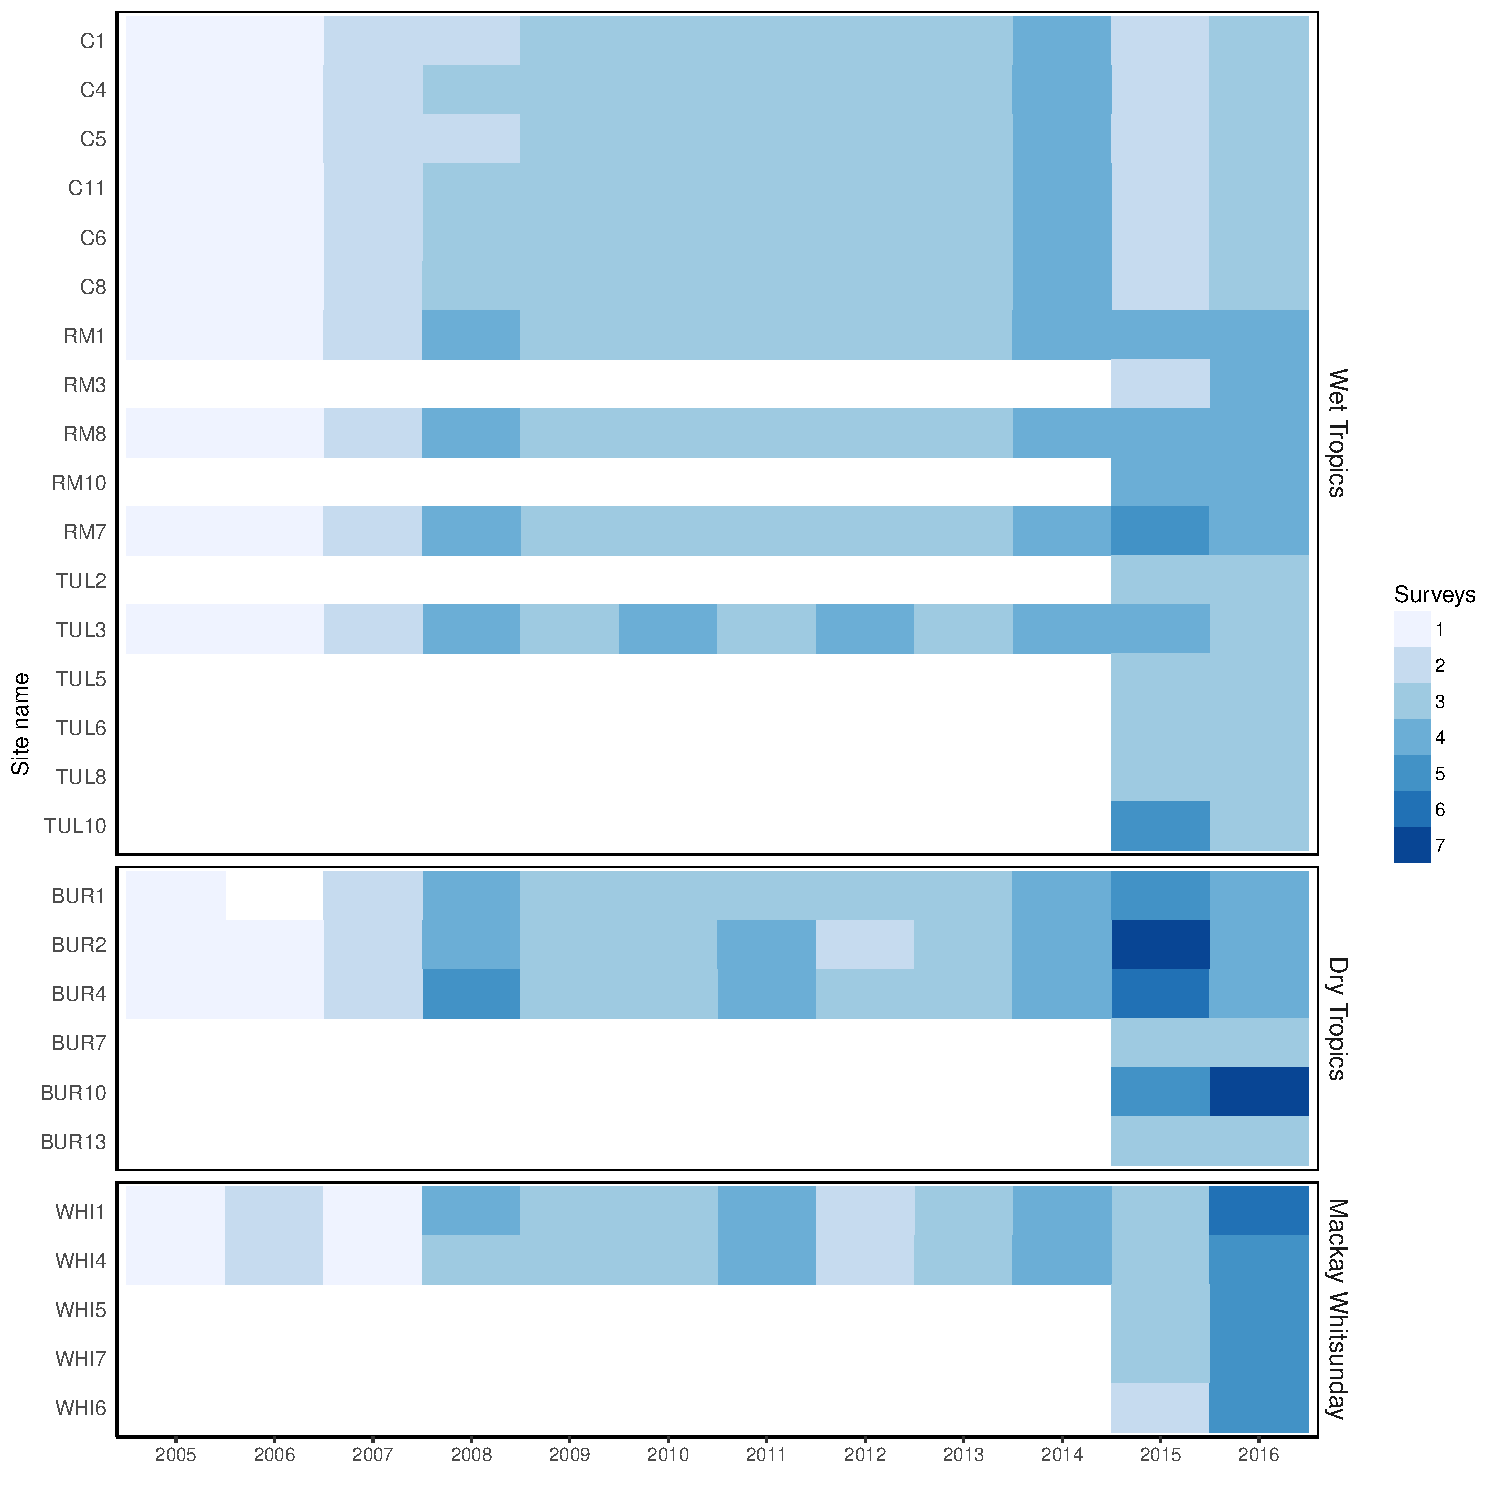
\includegraphics[width=1\linewidth]{figures/Maps/Insitu_sites/Samples_spatial_temporal.pdf}
\caption{Spatial and temporal distribution of AIMS insitu samples.  Sites names follow Great Barrier
Reef Marine Park Authority (GBRMPA) and sites are arranged north to south into the focal
Regions. Blue shading of tiles denotes the number of surveys conducted in the year at each
site.}\label{fig:AIMS_insitu_spatial_temporal}
\end{figure}
 
  \arrayrulecolor[rgb]{0.06,0.25,0.49}
 \LTcapwidth=\linewidth
 \setlength\aboverulesep{0pt}\setlength\belowrulesep{0pt}
 \setlength\cmidrulekern{1pt}\setlength\cmidrulewidth{1pt}
 \renewcommand\arraystretch{1.2}\setlength\tabcolsep{5pt}
 \begin{table}\caption{Measures collected in AIMS MMP insitu inshore water quality monitoring program.  NOx is the sum of NO$_2$ and NO$_3$.  Data used are annual means of depth weighted averages per site.}\label{tab:insitu.measures}
 %\begin{center}
 \scriptsize
 \begin{tabular}{
 !{\color[rgb]{0.06,0.25,0.49}\VRule[1pt]} p{10em}
 !{\color[rgb]{0.06,0.25,0.49}\vline} l
 !{\color[rgb]{0.06,0.25,0.49}\vline} p{15em}
 !{\color[rgb]{0.06,0.25,0.49}\vline} l
 !{\color[rgb]{0.06,0.25,0.49}\vline} l
 !{\color[rgb]{0.06,0.25,0.49}\vline} l
 !{\color[rgb]{0.06,0.25,0.49}\VRule[1pt]}
 }
 \arrayrulecolor[rgb]{0.06,0.25,0.49}\specialrule{1pt}{0pt}{0pt} %top border
 \rowcolor[rgb]{0.53,0.62,0.74} 
 \multicolumn{1}{!{\color[rgb]{0.06,0.25,0.49}\VRule[1pt]}l}{\whiteHeader{{Measure}}} & 
 \multicolumn{1}{l}{\whiteHeader{{Variable}}} & 
 \multicolumn{1}{l}{\whiteHeader{{Description}}} & 
 \multicolumn{1}{l}{\whiteHeader{{Abbreviation}}} & 
 \multicolumn{1}{l}{\whiteHeader{{Conversion}}} & 
 \whiteHeader{{Units}}\\ 
 \cmidrule{1-6} 
Chlorophyll-a & DRIFTCHL\_UGPERL.wm & Chlorophyll-a (µg/L) & chl & x1 & µgL^{-1} \\ 
   \cline{1-6}Total Suspended Solids & TSS\_MGPERL.wm & Suspended solids (mg/L) & nap & x1 & mgL^{-1} \\ 
   \cline{1-6}Secchi Depth & SECCHI\_DEPTH.wm & Secchi depth (m) & sd & x1 & m \\ 
   \cline{1-6}NOx & NOX.wm & Nitrite and Nitrate measured by microanalyser (µM/L) & NOx & x14 & µgL^{-1} \\ 
   \bottomrule
 \end{tabular}
 %\end{center}
 \end{table}


\clearpage

\subsection{AIMS FLNTU samples}
  
Combination continuous Flourometer and Turbidity Sensors (hereafter FLNTU) loggers were deployed at
15 of the AIMS MMP inshore water quality monitoring sites.
 
  \arrayrulecolor[rgb]{0.06,0.25,0.49}
 \LTcapwidth=\linewidth
 \setlength\aboverulesep{0pt}\setlength\belowrulesep{0pt}
 \setlength\cmidrulekern{1pt}\setlength\cmidrulewidth{1pt}
 \renewcommand\arraystretch{1.2}\setlength\tabcolsep{5pt}
 \begin{table}[h]\caption{Measures collected in AIMS MMP flntu inshore water quality monitoring program. Data used are daily means per site.}\label{tab:flntu.measures}
 %\begin{center}
 \scriptsize
 \begin{tabular}{
 !{\color[rgb]{0.06,0.25,0.49}\VRule[1pt]} p{10em}
 !{\color[rgb]{0.06,0.25,0.49}\vline} l
 !{\color[rgb]{0.06,0.25,0.49}\vline} p{15em}
 !{\color[rgb]{0.06,0.25,0.49}\vline} l
 !{\color[rgb]{0.06,0.25,0.49}\vline} l
 !{\color[rgb]{0.06,0.25,0.49}\vline} l
 !{\color[rgb]{0.06,0.25,0.49}\VRule[1pt]}
 }
 \arrayrulecolor[rgb]{0.06,0.25,0.49}\specialrule{1pt}{0pt}{0pt} %top border
 \rowcolor[rgb]{0.53,0.62,0.74} 
 \multicolumn{1}{!{\color[rgb]{0.06,0.25,0.49}\VRule[1pt]}l}{\whiteHeader{{Measure}}} & 
 \multicolumn{1}{l}{\whiteHeader{{Variable}}} & 
 \multicolumn{1}{l}{\whiteHeader{{Description}}} & 
 \multicolumn{1}{l}{\whiteHeader{{Abbreviation}}} & 
 \multicolumn{1}{l}{\whiteHeader{{Conversion}}} & 
 \whiteHeader{{Units}}\\ 
 \cmidrule{1-6} 
Chlorophyll-a & CHL\_QA\_AVG & ?? & chl & CHL\_QA\_AVG x1 & µgL^{-1} \\ 
   \cline{1-6}NTU & NTU\_QA\_AVG & ?? & ntu & NTU\_QA\_AVG x1 & NTU \\ 
   \bottomrule
 \end{tabular}
 %\end{center}
 \end{table}
 

\begin{figure}[ptbh] \includegraphics[width=1\linewidth]{figures/Exploratory_Data_Analysis/FLNTU/flntu_temporal\res.pdf}
\caption{Spatial and temporal distribution of AIMS FLNTU samples (Red: NTU, Green: Chlorophyll-a).
Sites names follow Great Barrier Reef Marine Park Authority (GBRMPA) and sites are arranged north to
south into the focal Regions.}\label{fig:flntu_temporal}
\end{figure}

\clearpage

\subsection{Remote sensing (BOM satellite)}

Daily (July 2002--Dec 2016, $1\times 1 km^2$ resolution) Moderate Resolution Imaging
Spectroradiometer (MODIS satellite) imagery (hereafter referred to as Satellite) data were obtained
by downloading NETCDF files from the thredds server (http://ereeftds.bom.gov.au/ereefs/tds/catalog/ereef/mwq/P1D/2002/catalog.html).
The data referred to herein relates to the individual measures considered in the data exploration
component of the project, and is distinct from the surface reflectance data used in the eReefs data
assimilation scheme discussed below in section \ref{sec:eReefs}.

  \arrayrulecolor[rgb]{0.06,0.25,0.49}
 \LTcapwidth=\linewidth
 \setlength\aboverulesep{0pt}\setlength\belowrulesep{0pt}
 \setlength\cmidrulekern{1pt}\setlength\cmidrulewidth{1pt}
 \renewcommand\arraystretch{1.2}\setlength\tabcolsep{5pt}
 \begin{table}[h]\caption{Measures collected from MODIS satellite imaging. Data used are daily means per pixel. Variable and Description pertain to the eReefs source.  Conversion indicates the conversion applied on data to conform to threshold Units.  Abbreviation provides a consistent key accross data. MIM refers to the robust and scalable matrix inversion method used to handle the variability in optical properties of satellite imagery.}\label{tab:satellite.measures}
 %\begin{center}
 \scriptsize
 \begin{tabular}{
 !{\color[rgb]{0.06,0.25,0.49}\VRule[1pt]} p{10em}
 !{\color[rgb]{0.06,0.25,0.49}\vline} l
 !{\color[rgb]{0.06,0.25,0.49}\vline} p{20em}
 !{\color[rgb]{0.06,0.25,0.49}\vline} l
 !{\color[rgb]{0.06,0.25,0.49}\vline} l
 !{\color[rgb]{0.06,0.25,0.49}\vline} l
 !{\color[rgb]{0.06,0.25,0.49}\VRule[1pt]}
 }
 \arrayrulecolor[rgb]{0.06,0.25,0.49}\specialrule{1pt}{0pt}{0pt} %top border
 \rowcolor[rgb]{0.53,0.62,0.74} 
 \multicolumn{1}{!{\color[rgb]{0.06,0.25,0.49}\VRule[1pt]}l}{\whiteHeader{{Measure}}} & 
 \multicolumn{1}{l}{\whiteHeader{{Variable}}} & 
 \multicolumn{1}{l}{\whiteHeader{{Description}}} & 
 \multicolumn{1}{l}{\whiteHeader{{Abbreviation}}} & 
 \multicolumn{1}{l}{\whiteHeader{{Conversion}}} & 
 \whiteHeader{{Units}}\\ 
 \cmidrule{1-6} 
Chlorophyll-a & Chl\_MIM} & Near surface concentration based on empirical relationship established between in situ measurements and blue-to-green band ratios & chl & Chl\_MIM} x1 & µgL^{-1} \\ 
   \cline{1-6}Non-Algal Particles & Nap\_MIM} & Total suspended solids based on relationship established between in situ measurements and the absorption concentration of non-algal particles & nap & Nap\_MIM} x1 & mgL^{-1} \\ 
   \cline{1-6}Secchi Depth & SD\_MIM} & Secchi depth based on empirical relationship established between in situ measurements and estimated depth at which 10\% of surface light still available & sd & SD\_MIM} x1 & m \\ 
   \bottomrule
 \end{tabular}
 %\end{center}
 \end{table}


 

%\subsection{eReefs assimilated model}

\subsection[eReefs coupled hydrodynamic]{eReefs coupled hydrodynamic - biogeochemical model}\label{sec:eReefs}

\begin{itemize}
\item \textcolor{red}{We need a table that specifies and explains the naming of the various
    eReefs models and where they are available}
\end{itemize}

The eReefs coupled hydrodynamic, sediment and BGC modelling system involves the application of a
range of physical, chemical and biological process descriptions to quantify the rate of change of
physical and biological variables (Fig.~\ref{fig:bgc}, \citet{Schiller14}). The processes
descriptions are generally based either on a fundamental understanding of the process (such as the
effect of gravity on circulation) or measurements when the process is isolated (such as the maximum
division rate of phytoplankton cells at 25$^{\circ}$C in a laboratory mono-culture). The model also
requires as inputs external forcings, such as observed river flows and pollutant loads. Thus, the
model can be run without observations from the marine environment and in this mode is quite skilful
(\citet{Skerratt18} and below). This mode which does not use observations from the marine
environment as the simulation is undertaken is referred to as the non-assimilating simulation. Most
of the eReefs marine biogeochemical simulations are non-assimilating.

\begin{figure}[thb]
\begin{center}
\resizebox{5in}{!}{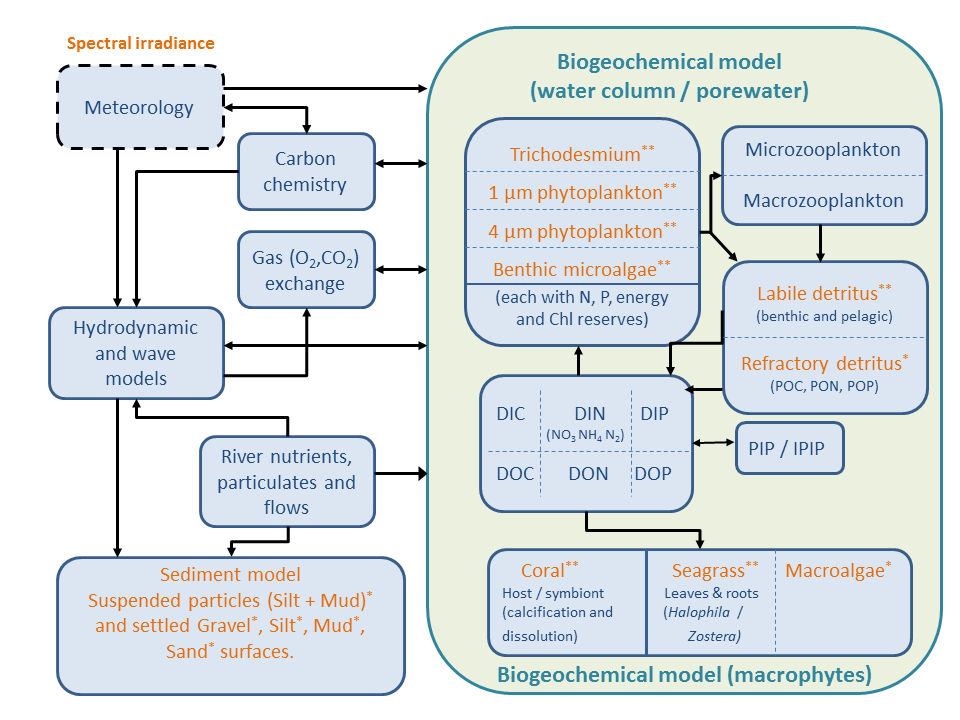
\includegraphics{figures/Mark/ereefsbgcdiagram4emlyn.png}}
\caption{Schematic showing eReefs coupled hydrodynamic biogeochemical model.}
\label{fig:bgc}
\end{center}
\end{figure}

\begin{figure}[thb]
\begin{center} \resizebox{5in}{!}{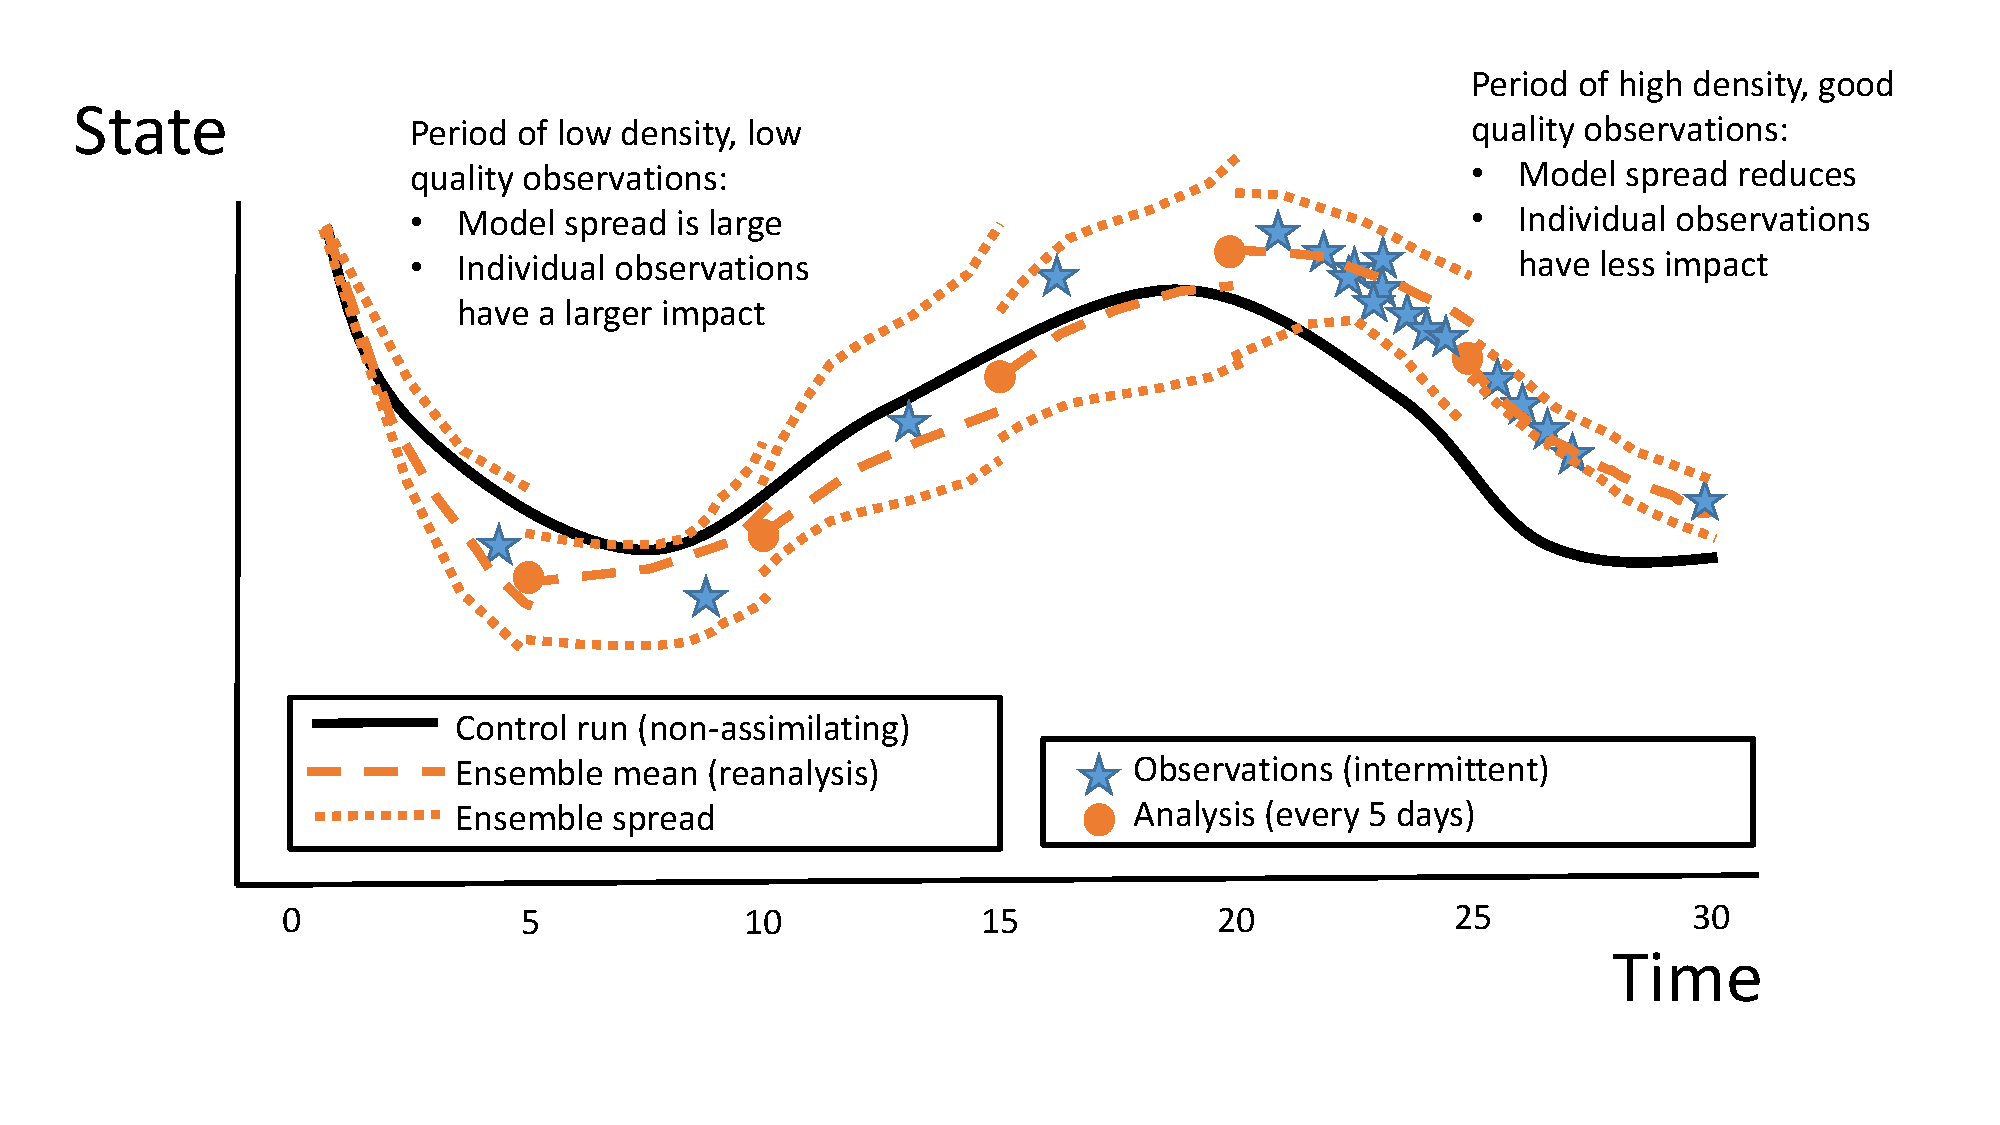
\includegraphics{figures/Mark/EnKFschematic.pdf}}
\caption{Schematic showing the evolution of the model ensemble over 6 assimilation cycles using the
Ensemble Karman Filter (EnKF) system. The non-assimilating control run (black line) is capturing the
gross cycle in the observations (blue stars), but errors remain that observations can constrain. At
the initial time, all ensemble members, and the control run, have similar values.  In the first five
days the 108 members develop a spread, with the control run being different to the ensemble mean,
but within the ensemble spread. At 5 days, the first state updating occurs. In the first 5 days
there was only one observations, being above the ensemble mean. At day 5, a new state for the entire
ensemble is calculated (the analysis being the mean of the updated ensemble) based on the mismatch
between the ensemble members and observations. The updated state is closer to the model if the
ensemble spread is small, or to the observations if they are dense with few errors. At day 5,
because of the small positive mismatch, the ensemble spread is only slightly narrowed, and the mean
increased. The ensemble members all restart from these new updated states. The next four analysis
steps proceed much like the first. For the fifth analysis step, high density observation were
available over the previous 5 days, so the analysis is weighted heavily toward the observations, and
the model spread is constrained significantly. Looking at the error between the ensemble mean and
the observations over the entire period we see that the data assimilation system has provided an
improved estimate of the state (the mean of the ensemble) relative to the control run, and achieved
this using the model that contains the processes we understanding to describe system.}
\label{fig:da}
\end{center}
\end{figure}

Despite being already skilful, the predictive skill of the model can be improved by assimilating
marine observations into an ensemble (i.e. a large number (108) of similar but not identical) of
model simulations. The form of data assimilation we chose, and that is commonly used in weather
forecasting, involves updating of the state of the model as the simulation progresses
(Fig.~\ref{fig:da}). State updating involves first looking for a mismatch between the state of the
ensemble members and the observations over the previous 5 days. Ocean colour, the observation of
water-leaving irradiance at 8 individual wavebands, provides the only data set with sufficient
temporal (daily) and spatial (1 km) resolution, providing upwards of 13 million pixels on a
cloud-free day. For this comparison, we have chosen to use the mismatch between the model's
prediction of the ratio of the water-leaving irradiance at 443 nm (blue) and 551 nm (green) and the
observation of the same quantities from the MODIS sensor on NASA's Aqua satellite. The eReefs
biogeochemical model is the first published model to assimilate raw ocean colour observations
\citep{Jones16}. The data assimilation algorithm uses the model-observation mismatch, as well as
statistically-quantified dynamical properties of model, to periodically alter the values in the 108
member ensemble, resulting the ensemble mean gaining a closer match to the observations. The outcome
of this modelling system is referred to in the field of data assimilation as a reanalysis.

Below we describe the model itself, and then particular data assimilation system.

\subsubsection{eReefs coupled model description and forcing}

The hydrodynamic model is a fully 3-D finite-difference baroclinic model based on the 3-D equations
of momentum, continuity and conservation of heat and salt, employing the hydrostatic and Boussinesq
assumptions \citep{Herzfeld06,Herzfeld15a}. The sediment transport model adds a multilayer sediment
bed to the hydrodynamic model grid and simulates sinking, deposition and resuspension of multiple
size classes of suspended sediment \citep{Margvelashvili09,Margvelashvili16}. The complex BGC model
simulates optical, nutrient, plankton, benthic organisms (seagrass, macroalgae and coral), detritus,
chemical and sediment dynamics across the whole GBR region, spanning estuarine systems to
oligotrophic offshore reefs (Fig.~\ref{fig:bgc}, \citet{Baird16a}). An expanded description of the
BGC model is given in Appendix A, with a brief description of the optical model in Appendix
B. Briefly, the BGC model considers four groups of microalgae (small and large phytoplankton,
Trichodesmium and microphytobenthos), two zooplankton groups, three macrophytes types (seagrass
types corresponding to Zostera and Halophila, macroalgae) and coral communities.

Photosynthetic growth is determined by concentrations of dissolved nutrients (nitrogen and
phosphorous) and photosynthetically active radiation. Microalgae contain two pigments (chlorophyll a
and an accessory pigment) and have variable carbon : pigment ratios determined using a
photoadaptation model (described in \citet{Baird13}. Overall, the model contains 23 optically active
constituents (\citet{Baird16a}; and Appendix A).

The model is forced with freshwater inputs at 21 rivers along the GBR and the Fly River in southwest
Papua New Guinea. River flows are obtained from the DERM (Department of Environment and Resource
Management) gauging network. Nutrient concentrations flowing in from the ocean boundaries were
obtained from the CSIRO Atlas of Regional Seas (CARS) 2009 climatology \citep{Ridgway02}.

The nutrient loads (TSS, PN, PP, DIN,DIP) for the 21 rivers were obtained from the process-based
Source models used for Paddock 2 Reef (P2R) load reduction estimates \citep{Waters14}. The P2R
represenst land uses and landscape processes in a variety of ways, often based upon spatially
explicit farm-scale models that are included through a system of bespoke pre-processing and transfer
tools. These P2R Source models also include flow related in-stream processing of pollutants, thus
altering loads as fluxes transfer throughout the network. P2R modelling includes scenarios designed
to represent ‘baseline’ (or ‘current condition’) and ‘pre-development’ catchment loads. In this
report we only use 'baseline' condition. The reliance of the base P2R Source models on external,
farm scale sub-models, means that they cannot be easily modified to extend the period covered by the
report card. Thus we only use the P2R outputs from Jan 2011 - July 2014.

In order to provide daily timeseries predictions of pollutant loads past July 2014, the reliance on
external sub-models was replaced by pollutant generation models that estimate daily loads through
monthly varying concentrations (‘EMC/DWC’). The particular concentration values for each pollutant
for each Functional Unit (FU) within each subcatchment have been calculated by analysing the monthly
runoff volumes and pollutant loads from the P2R Source models defined in \citet{Waters14}. The
network transport and in-stream processing mechanisms are unaltered from the base P2R Source
models. These monthly concentration pollutant generation models allow the model predictions to be
extended by providing updated rainfall runoff model inputs (i.e. the runoff of the day), without the
need to also update many thousands of farm scale sub-models. Simple comparisons of predicted loads
indicates that the monthly varying concentration approach works reasonably well for sediment and
associated particulate nutrient, and less well for pollutants that are usually reliant on farm scale
representation of management inputs.

\subsubsection{Assimilation system}

%\subsubsection{Assimilation of ocean colour}
\paragraph{Assimilation of ocean colour}

Ocean colour was chosen as the data set to assimilate due to its availability over the entire GBR at
high temporal and spatial density. Ocean colour has often been used for biogeochemical data
assimilation \citep{Kidston13}. In global biogeochemical data assimilation applications, the
observation - model mismatch used has often been satellite estimates of \textit{in situ} chlorophyll
concentration versus model predicted chlorophyll concentration \citep{Ford12}. This approach is
problematic in coastal waters such as the GBR, where chlorophyll concentration is often
overestimated by satellite algorithms due to bottom reflectance or absorption by non-phytoplankton
components \citep{Schroeder12b}. So it is not possible in this application to base the data
assimilation system on the mismatch of model chlorophyll against satellite estimates of \textit{in
situ} chlorophyll. Instead, we have pioneered the use of remote-sensing reflectance as the variable
to determine the mismatch between the observed and modelled quantities \citep{Jones16}.

Remote-sensing reflectance, $R_{rs}$, is the ratio of the water-leaving irradiance in the direction
of a satellite to the water entering radiance. In this sense it is a 'raw' satellite
observation. The value of $R_{rs}$ varies with wavelength and is measured in sr$^{-1}$ (sr =
steradians, the SI unit of solid angle, where the solid angle in all direction on a spherical
surface is $4 \pi$ sr). In the open ocean at blue wavelengths the value is around 0.03 sr$^{-1}$
\citep{Baird16a}. That is, 3 \% of the light that entered the ocean within 1 m$^{2}$ emerged
travelling in the direction within a solid angle of 1 sr (i.e. $1 / 4 \pi$ of a sphere).

The model contains 23 optically active constituents (shaded orange in Fig.~\ref{fig:bgc}, see also
\citet{Baird16a}). For each of these constituents the optical model calculates the rate of
absorption, scattering and backscattering. To calculate $R_{rs}$ at the surface, we need to consider
the light returning from multiple depths, and from the bottom. Rather than using a computationally
expensive radiative transfer model, we approximate $R_{rs}$ based on an optical-depth weighted
scheme \citep{Baird16a}. The model sums the return from each depth (and the bottom) to give the
surface $R_{rs}$. As shown in \citet{Baird16a}, this calculation is sufficiently accurate that the
primary reason for the mismatch between observed and modelled $R_{rs}$ is errors in the coupled
hydrodynamic-biogeochemical model prediction of optically-active constituents. This is, of course,
the result we wanted - it means that when the assimilation system updates the optically-active
biogeochemical constituents in order to minimise the mismatch between observed and modelled
$R_{rs}$, it is changing the components of the model that have the greatest errors, and in doing so
improving the solution of those parts that we most care about - the optically-active components that
determine water clarity.

When testing the data assimilation system, we found that the best quantity to assimilate was the
ratio of the remote-sensing reflectance at 443 and 551 nm. In fact, this ratio is the same one used
in the NASA OC3M algorithm that we mentioned above is NOT a good measure of \textit{in situ}
chlorophyll in coastal waters! So how can it be that OC3M is a poor predictor of \textit{in situ}
chlorophyll in coastal waters, yet assimilating the mismatch between simulated OC3M and
satellite-observed OC3M achieves the best skill for \textit{in situ} chlorophyll when compared
against independent \textit{in situ} observations? The answer lies in that simulated OC3M is
calculated using the ratio of two simulated $R_{rs}$, in the same manner in which observed OC3M is
calculated using the ratio of two observed $R_{rs}$. Fig.~\ref{fig:OC3M} shows the \textit{in situ}
chlorophyll concentration, the simulated OC3M and the NASA observed OC3M for the Cape York region on
a relatively clear day.  The \textit{in situ} chlorophyll concentration in coastal regions along
this coast is $\sim 0.5$ mg m$^{-3}$ (Fig.~\ref{fig:OC3M} left). The simulated OC3M, calculated from
simulated $R_{rs}$, is greater along the coastal fringe due to the absorption of blue light from
CDOM, and addition bottom reflection of green light (Fig.~\ref{fig:OC3M} centre). The observed OC3M,
also affected by CDOM absorption and the bottom, looks more like the simulated OC3M than the
\textit{in situ} chlorophyll concentration (Fig.~\ref{fig:OC3M} right). Further, where there are
differences, the primary cause is the error in the simulated water-column optically-active
constituents like chlorophyll. Thus by producing the same simulated and observed quantity, we have
improved the ability of the assimilation system to update the optically-active model constituent
that is in error.

\begin{figure}[thb]
\begin{center} \resizebox{5in}{!}{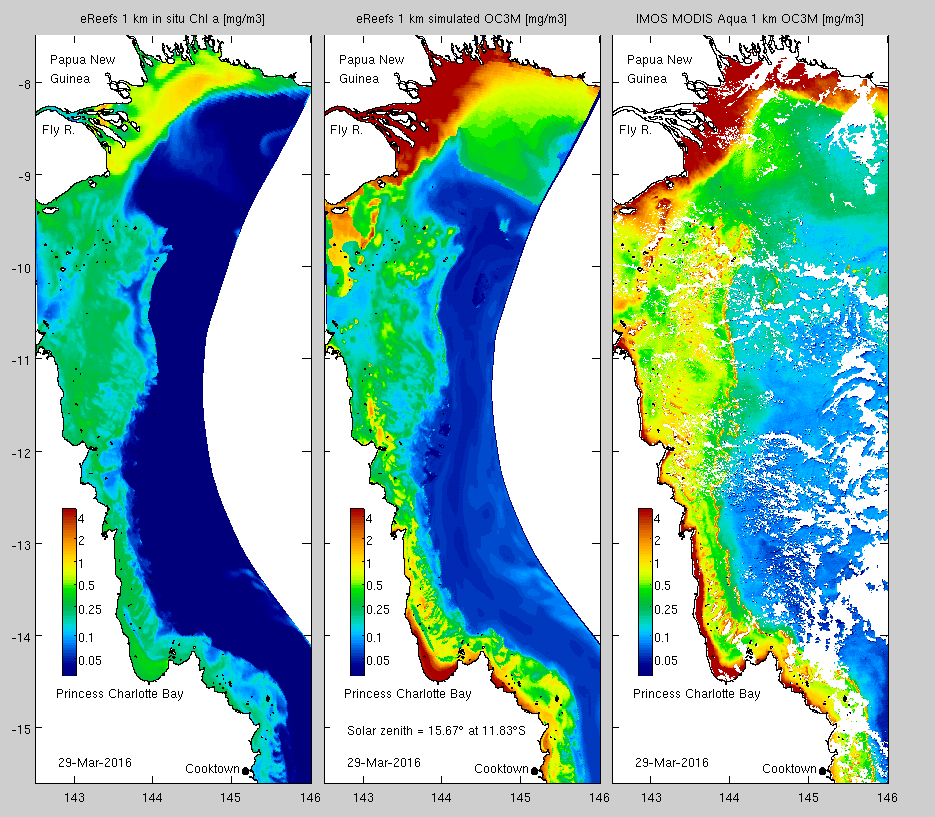
\includegraphics{figures/Mark/OC3M4reanalysis.png}}
\caption{Example of the estimates of OC3M in the Cape York region on the 29 March 2016 using the 1
km GBR1 model and the NASA Aqua MODIS sensor: \textit{in situ} chlorophyll concentration (left), the
simulated OC3M (centre) and the NASA observed OC3M (right).}
\label{fig:OC3M}
\end{center}
\end{figure}

OC3M uses the ratio of above-surface remote-sensing reflectance as a combination of three
wavelengths, $R'$, which is given by:
\begin{equation} R' = \log_{10} \left( \mathrm{max} \left[ R_{rs,443}, R_{rs,488} \right] /
R_{rs,551} \right)
\end{equation} The ratio $R'$ is used in the OC3M algorithm to estimate surface chlorophyll,
$\mathrm{Chl}_{OC3}$, with coefficients from the 18 March 2010 reprocessing:
\begin{equation} \mathrm{Chl}_{OC3} = 10^{0.283 + R' \left(-2.753 + R' \left( 1.457 + R' \left(0.659
- 1.403 R' \right) \right) \right)}
\end{equation} obtained from \texttt{oceancolor.gsfc.nasa.gov/REPROCESSING/R2009/ocv6/}. Using, OC3M
we gain the benefit of assimilating directly the mismatch between the simulated OC3M (based on
simulated remote-sensing reflectance) and the observed remote-sensing reflectance; and we use a
quantity that has meaning in the water quality community (mass concentration of chlorophyll). To
re-state, because we use the simulated remote-sensing reflectance to calculate OC3M, the system is
not affected by the inaccuracies in the relationship between in situ chlorophyll and
satellite-derived OC3M. And our assimilation system's prediction of chlorophyll is the simulated
\textit{in situ} chlorophyll concentration (and not OC3M).

The accuracy of the modelling systems also requires that the model and observations are closely
matched in space and time. This is because remote-sensing reflectance is a function of solar angle
(and therefore time of day), and because the optical properties of coastal waters can vary quickly
due to a range of processes such as phytoplankton chlorophyll synthesis, movement of fronts, wind
driven-upwelling, river plume structure changes etc. We used the flexible outputting time of the
model, and the asynchronous assimilation routines in the EnKF-C package \citep{Sakov17}, to closely
align the observations and models. In doing so we were able to meet the $\pm 30$ minutes matching
requirements used for the calibration / validation of ocean colour satellite products.

The Aqua satellite overpasses the GBR between 1130 and 1530 locally. In order to match the model
output to within 30 minutes of the overpass, the model remote-sensing reflectance was output at
1200, 1300, 1400 and 1500 daily. For the calculations of remote-sensing reflectance, the water
column calculations of the light field (and $R_{rs}$) was redone on the output time assuming the
entire grid is at 150$^{\circ}$E, while infact it varies from 142$^{\circ}$31'E to
156$^{\circ}$51'E. Thus the maximum error in calculating solar angle for the purposes of outputting
$R_{rs}$, in the Torres Strait, is about 30 minutes (this small error will be corrected in the next
phase of eReefs). The light field calculation was also done at wavelengths at the centre of the
MODIS ocean colour bands to avoid any small interpolations from the spectrally-resolved model that
has a 20 nm resolution.

The observations also need to be spatially aligned. The observations are at approximately $\sim$1 km
resolution (up to 2 km on the edges of the swath), with location varying spatially with each
different satellite swath. Meanwhile the model cells are stationary, are $\sim$ 16 km$^2$, and are
defined on the curvilinear grid. The observations are grouped into a "superobservation" for each
model cell. The superobservation contains all observations that were closer to a particular cell
centre than any other cell centre. The position of the superobservation is the mean of the
observations it is composed of, and will be close to, but not exactly the same, as the location of
the cell centre. The assimilation system then accounts for the now small misalignment in time and
space when considering the mismatch between the model and observation.

%\subsubsection{Ensemble member design}
\paragraph{Ensemble member design}

The assimilation system used in this study is the Determininstic Ensemble Kalman Filter (DEnKF) that
requires an ensemble of model runs that approximate the uncertainty in the model solution.  The
uncertainty in the model solution arises from uncertainty in the model initial conditions, boundary
conditions, surface forcing and model parameterisations.  The ensemble members differ in the values
of the quadratic mortality rate coefficient of small zooplankton, in the loads of nutrients
delivered in the rivers (as a multiple of the SOURCE catchments specified loads), and in the PAR
light forcing (again as a multiple of the Bureau of Meteorology short wave radiation
prediction). These relatively small differences, which are undertaken on the most uncertain
biological parameter, and most sensitive forcing paramaters, provide a spread of ensemble members
that the Karman Filter can operate on.

For a further description of the numerical schemes in the assimilation system see \citep{Jones16}. A
number of modifications have been made to improve the accuracy and efficiency of the system,
including transferring the the EnKF-C software.

\subsubsection{Summary results}

The non-assimilating version of the model has been compared to observations previously (ereefs.info,
\citet{Baird16a} and \citet{Skerratt18}). The results produced in the reanalysis are compared
directly to observations in the attached 100 page appendix showing comparisons to hundreds of
time-series. Further, later components of this document compare the metric calculated using the
non-assimilating model, the assimilating model, satellite observations and \textit{in situ}
observations. Here we will just show a few snapshot results to aid in the understanding of the
performance of the data assimilation relative to the non-assimilating run.

%\subsubsection{Assessment of chlorophyll concentration at MMP sites}
\paragraph{Assessment of chlorophyll concentration at MMP sites}

In our assessment of the skill of the eReefs biogeochemical models, we have considered the most
important property to be the prediction of \textit{in situ} chlorophyll concentration at the MMP
sites. For this there are two measures - the chlorophyll extractions at the sampling sites, and the
calibrated chlorophyll fluorescence on the moorings.  While the extractions are considered the most
accurate, the fluorescence time-series is continuous. When the two are lined up in time (they are
slightly separated in space), the mismatch between the observed chlorophyll extractions and the
observed chlorophyll fluorescence is 0.2 mg m$^{-3}$. We use this 0.2 mg m$^{-3}$ as indicative of
the error of the observations.

It is important to note that the \textit{in situ} chlorophyll concentration observations were not
assimilated into the model. That is, they were observation withheld just for the model
assessment. In fact, the mismatch between observed and modelled quantities used in the assimilation
system is neither an \textit{in situ} measurement, nor a chlorophyll concentration. The assimilated
quantity was the ratio of remote-sensing reflectance at blue and green wavelengths. Thus, we can be
confident that if the assimilation system has improved the prediction of \textit{in situ}
chlorophyll concentration then it has improved the overall biogeochemical model.

At 13 of the 14 MMP site, the assimilation of satellite-observed remote-sensing reflectance improved
the prediction \textit{in situ} chlorophyll concentration (Fig.~\ref{fig:RMSerror}, top). On average
the assimilation reduced the error from 0.34 to 0.29 mg m$^{-3}$, bring it 30 \% closer to the
observation error (the limit of our ability to quantify an improvement in the model). The worst two
site remained the most coastal sites, Geoffrey Bay and Dunk Island, for which the 4 km model poorly
resolves local processes, and for which the assimilation system would provide little information to
water column due to the optically-shallow and complex waters. The best site was Double Cone Island
off Airlie Beach. At Double Cone Island, a time-series shows the improvement in the chlorophyll
fluorescence due to the assimilation (Fig.~\ref{fig:RMSerror}, bottom). During a particularly
cloud-free period in the second half of 2015, the assimilation system does a remarkable job of both
removing model bias and capturing variability in the model.


\begin{figure}[thb]
\begin{center} \resizebox{5in}{!}{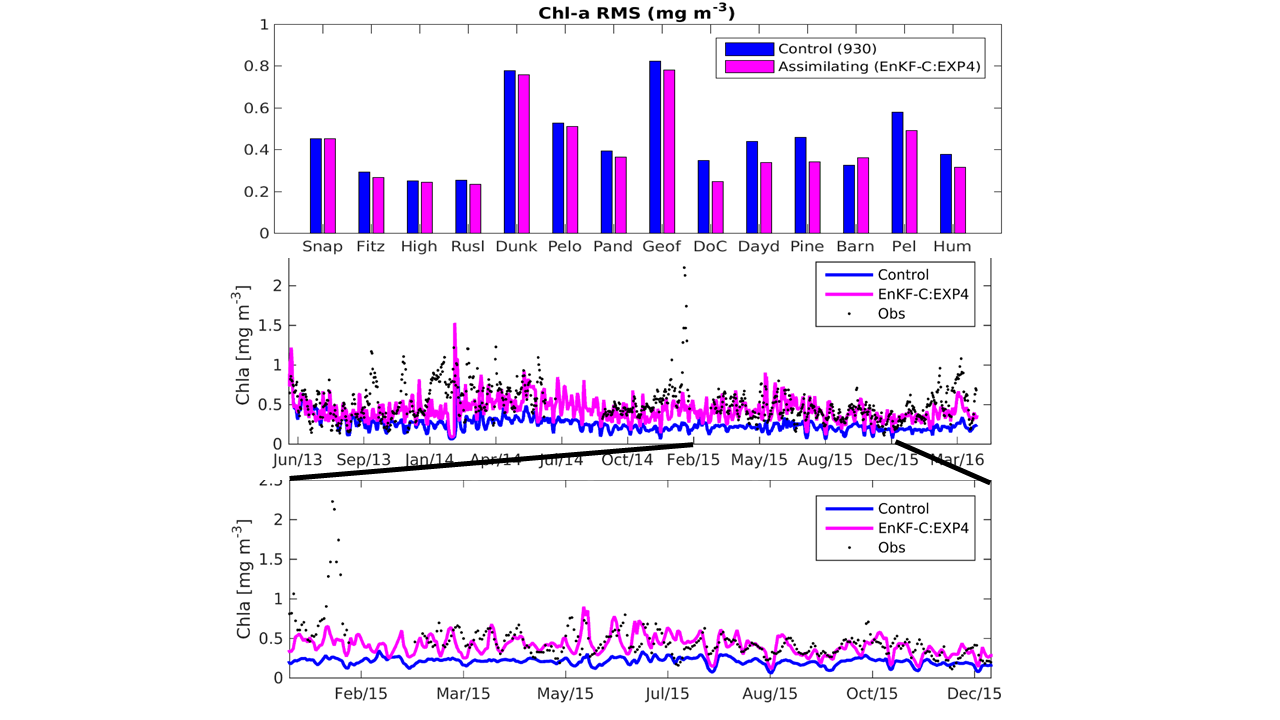
\includegraphics{figures/Mark/reanalysisRMSerror.png}}
\caption{Comparison of the non-assimilating (blue) and assimilating (pink) runs at the MMP
sites. The instantaneous state root mean square error at the 14 MMP sites (top). The approximate
error in the observations is 0.2 mg m$^{-3}$. At Double Cone Island in the Whitsundays (off Airlie
Beach), a time-series of the observations (black dots) and simulations is shown for the whole
simulations (centre) and the a 1 year period (bottom).}
\label{fig:RMSerror}
\end{center}
\end{figure}


% **Mark to provide a brief description**.

\arrayrulecolor[rgb]{0.06,0.25,0.49}
\LTcapwidth=\linewidth
\setlength\aboverulesep{0pt}\setlength\belowrulesep{0pt}
\setlength\cmidrulekern{1pt}\setlength\cmidrulewidth{1pt}
\renewcommand\arraystretch{1.2}\setlength\tabcolsep{5pt}
\begin{table}[ht]\caption{eReefs regional biogeochemical simulation catalog.}\label{tab:ereefs}
  \scriptsize
  \begin{tabular}{
    !{\color[rgb]{0.06,0.25,0.49}\VRule[1pt]} p{15em}
    !{\color[rgb]{0.06,0.25,0.49}\vline}l
    !{\color[rgb]{0.06,0.25,0.49}\vline}l
    !{\color[rgb]{0.06,0.25,0.49}\vline}l
    !{\color[rgb]{0.06,0.25,0.49}\vline}l
    !{\color[rgb]{0.06,0.25,0.49}\vline}l
    !{\color[rgb]{0.06,0.25,0.49}\VRule[1pt]}
    }
    \arrayrulecolor[rgb]{0.06,0.25,0.49}\specialrule{1pt}{0pt}{0pt} %top border
    \rowcolor[rgb]{0.53,0.62,0.74}
    \multicolumn{1}{!{\color[rgb]{0.06,0.25,0.49}\VRule[1pt]} p{15em}}{\whiteHeader{{Simulation name}}} & 
    \multicolumn{1}{l}{\whiteHeader{{Projects}}}&
    \multicolumn{1}{l}{\whiteHeader{{Date range}}}&
                                                    \multicolumn{1}{l}{\whiteHeader{{Delivery}}}&
                                                                                                  \whiteHeader{{Notes/Improvements}}\\
    \cmidrule{1-5}
    GBR4\_H1p85\_B1p0\_Cbas\_Dhnd & SIEF & Jan 1, 2011 -- Jun 30, 2014 & Available on NCI & Simulation delivered as part of SIEF project (previously known as 926). Skill assessment available in SIEF report.\\
    \cline{1-5}& & & &\\
    \cline{1-5}& & & &\\
    \bottomrule
  \end{tabular}
\end{table}


In this context, the \textbf{eReefs} model refers to the
GBR4\_H2p0\_B1p9\_Chyd\_Dran model (see Table\ref{tab:ereefsModels}) for the catalog and model descriptions and
Table\ref{tab:ereefs.measures} for a description of the variables and processing).

This source of data only extends back to 2014. Whilst the eReefs GBR4\_H2p0\_B1p9\_Chyd\_Dran model technically does
contain 2013 calendar year data, the current project partitions time into water years in which the
full 2013 water year starts in October 2012.  Therefore as the 2013 is not a complete 12 months of
data, it is excluded from analyses. Unfortunately, this means that any signals associated with the
2010-2011 floods are unavailable.
 
  \arrayrulecolor[rgb]{0.06,0.25,0.49}
 \LTcapwidth=\linewidth
 \setlength\aboverulesep{0pt}\setlength\belowrulesep{0pt}
 \setlength\cmidrulekern{1pt}\setlength\cmidrulewidth{1pt}
 \renewcommand\arraystretch{1.2}\setlength\tabcolsep{5pt}
 \begin{table}[h]\caption{Measures collected from eReefs assimilated model. Data used are daily means per pixel. Variable and Description pertain to the eReefs source.  Conversion indicates the conversion applied on data to conform to threshold Units.  Abbreviation provides a consistent key accross data. }\label{tab:ereefs.measures}
 %\begin{center}
 \scriptsize
 \begin{tabular}{
 !{\color[rgb]{0.06,0.25,0.49}\VRule[1pt]} p{10em}
 !{\color[rgb]{0.06,0.25,0.49}\vline} l
 !{\color[rgb]{0.06,0.25,0.49}\vline} p{20em}
 !{\color[rgb]{0.06,0.25,0.49}\vline} l
 !{\color[rgb]{0.06,0.25,0.49}\vline} l
 !{\color[rgb]{0.06,0.25,0.49}\vline} l
 !{\color[rgb]{0.06,0.25,0.49}\VRule[1pt]}
 }
 \arrayrulecolor[rgb]{0.06,0.25,0.49}\specialrule{1pt}{0pt}{0pt} %top border
 \rowcolor[rgb]{0.53,0.62,0.74} 
 \multicolumn{1}{!{\color[rgb]{0.06,0.25,0.49}\VRule[1pt]}l}{\whiteHeader{{Measure}}} & 
 \multicolumn{1}{l}{\whiteHeader{{Variable}}} & 
 \multicolumn{1}{l}{\whiteHeader{{Description}}} & 
 \multicolumn{1}{l}{\whiteHeader{{Abbreviation}}} & 
 \multicolumn{1}{l}{\whiteHeader{{Conversion}}} & 
 \whiteHeader{{Units}}\\ 
 \cmidrule{1-6} 
Chlorophyll-a & Chl\_a}\_um & Sum of Chlorophyll concentration of four microalgae types ($mg/m^3$) & chl & Chl\_a}\_um x1 & µgL^{-1} \\ 
   \cline{1-6}Non-Algal Particles & EFI & EFI = NAP and is the sum of Mud and Fine Sediment & nap & EFI x1000 & mgL^{-1} \\ 
   \cline{1-6}Secchi Depth & Kd\_490} & Kd\_490 is calculated from the scattering and absorbing properties of all optical-active constituents, and includes the cosine zenith angle on vertical attenuation. & sd & 1/Kd\_490} & m \\ 
   \cline{1-6}NOx & NO3 & Concentration of Nitrate. As Nitrite is not represented in the model, NO3 = $[NO^-_3] + [NO^-_2]$ ($mg/m^3$) & NOx & NO3 x1 & µgL^{-1} \\ 
   \bottomrule
 \end{tabular}
 %\end{center}
 \end{table}
    
      

\subsection{eReefs926}

In this context, the \textbf{eReefs926} model refers to the
GBR4\_H1p85\_B1p0\_Cbas\_Dhnd  model (see Table\ref{tab:ereefsModels}). This model provides alternative formulation
and importantly does extend back to the full 2013 water year thereby providing some coverage closer
to the 2010-2011 flood period.

Variables used as per Table~\ref{tab:ereefs.measures}.

\subsection{Thresholds}

An environmental health metric represents the state or condition relative to some reference,
threshold or expectation.  Most of the current water quality indices compare values to a set of
specifically selected \textit{guidelines}.  These guidelines are either formulated specifically from
long-term historical data appropriate to the spatial and temporal domain of interest or else are
based on ANZEC guidelines \citep{ANZEC-2000}.
 
Typically there are strict guidelines on how these guidelines should be applied.  In particular, the
guidelines associated with various measures used in various report cards throughout the Great
Barrier Reef should be applied to annually aggregated data - not individual observations.  Since
this project intends to generate indices on the scale of individual observations, we have decided to
refer to the guidelines as \textit{thresholds} so as to avoid contradicting the terms of use of
guidelines..
 
The thresholds used for each Measure within each Region and Water body are indicated in
Table~\ref{tab:thresholds} (page~\pageref{tab:thresholds}).  Note, that whilst the application of
seasonal thresholds could potentially remove some uncertainty, in the absence of clear consensus on
how to define wet and dry seasons and what the associated set of thresholds would be, seasonal
thresholds are not used in this project.
